\chapter{Splay Trees}

Gli splay trees sono delle strutture \textbf{auto bilancianti}, questi implementano $M$ operazioni consecutive di \textbf{ricerca, inserimento e cancellazione} in un tempo $O(MlogN)$ dove $N$ rappresenta il numero di inserimenti in un albero inizialmente vuoto. 
Alla base di questa struttura dati, vi è l'idea che i nodi che sono stati ricercati una volta, saranno ricercati ancora in un breve tempo. Di conseguenza, si cerca di avvicinare i nodi che si incontrano alla radice per velocizzare questo accesso. Per fare ciò, il modo più semplice è quello di continuare a fare rotazioni da basso verso l'alto lungo tutto il cammino. Tuttavia, questo metodo necessita di qualche piccola modifica per funzionare correttamente, infatti, possiamo analizzare la complessità senza modifiche e vedere cosa succede. 

Immaginiamo di avere N inserimenti e di contare il costo di un'operazione in base al numero di rotazioni che è necessario fare per portare un nodo alla radice. Prendiamo in considerazione adesso la sequenza di operazioni < insert(1), insert(2),...,insert(n), search(1), search(2),..., search(n) >. Per quando riguarda gli inserimenti, avremo che la complessità totale sarà $\theta(N)$ poiché, ad ogni inserimento faremo almeno una rotazione. Le cose si complicano quando cominciamo ad effettuare le ricerche:
\begin{figure}[H]
    \centering
    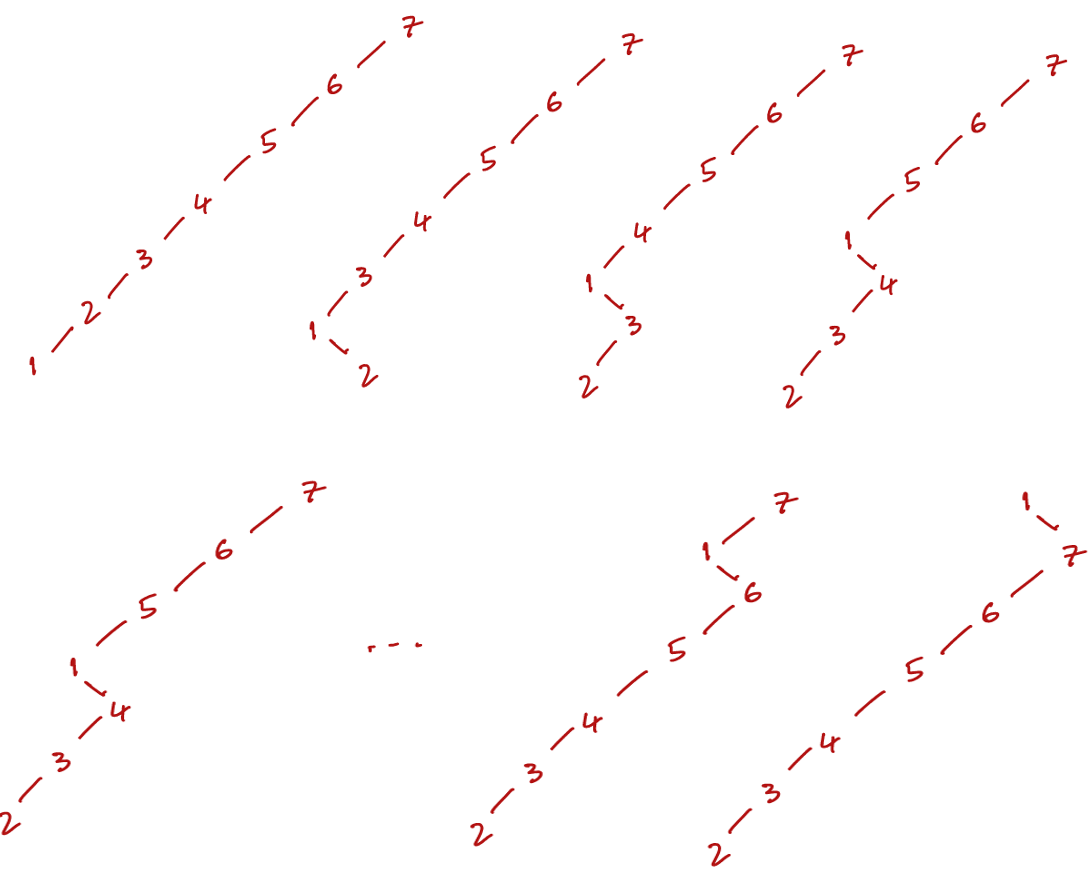
\includegraphics[width=0.65\linewidth]{Images/capitolo_1_2/albero_search.png}
    \label{fig:albero_ricerca}
\end{figure}

Come possiamo vedere, la ricerca di 1 ha un costo di N-1 rotazioni e sarà lo stesso per la ricerca di 2. Vedremo però, che passando alla ricerca di tre il numero di rotazioni sarà N-2, poi per 4 sarà N-3 ecc. In totale, avremo la complessità per la seconda parte delle operazioni di $\sum_i^ni-1 $, da cui avremo all'incirca una complessità totale di $\theta(N^2)$. 

\section{Zig, Zig-Zag, Zig-Zig}
Per risolvere questo problema, introduciamo alcune casistiche utili per l'analisi della complessità. Queste sono \textbf{Zig, Zig-Zag e Zig Zig}, che possiamo tranquillamente vedere in figura. 
\begin{figure}[H]
    \centering
    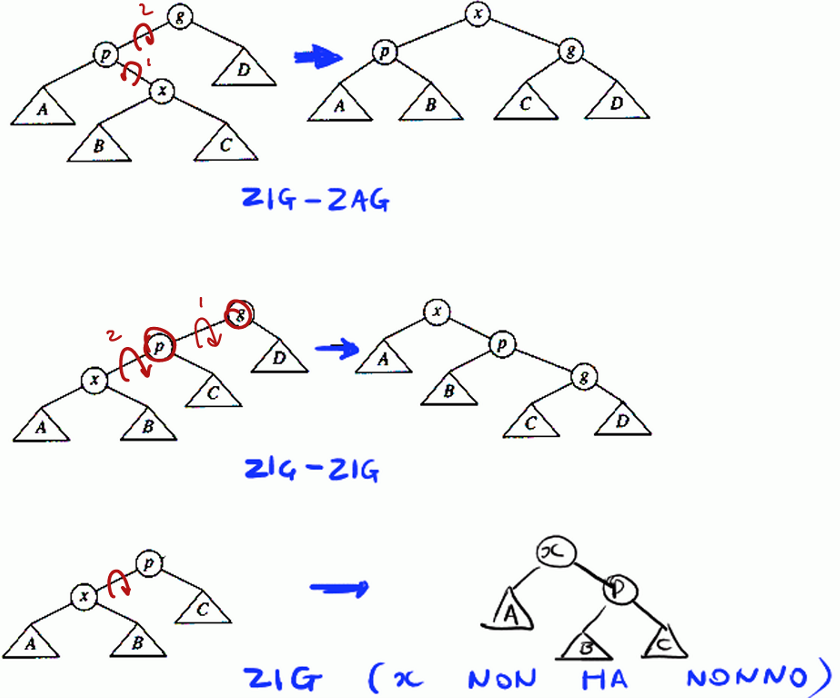
\includegraphics[width=1\linewidth]{Images/capitolo_1_2/zig_zigzag_zigzig.png}
    \label{fig:zig_zag_zig}
\end{figure}

In pratica, l'unica cosa che cambia è che nel caso simmetrico, anziché partire dal basso verso l'alto, la prima rotazione sarà quella in alto e poi faremo quella in basso. Questo cambiamento, seppure molto piccolo, cambia tutto e fa sì che l'albero riesca a bilanciarsi nella maggior parte dei casi.
Introduciamo quindi le operazioni che possono essere eseguite:
\begin{itemize}
    \item \textbf{Splay(x,T):} Si cerca sull'albero T l'elemento x mediante ricerca binaria. Dopodiché, a partire dal nodo ove la ricerca si è fermata, si applicano le operazioni di zig, zig-zag e zig-zig necessarie.
    \item \textbf{Insert(x,T):}: Si esegue una Splay(x,T) e, una volta che l'elemento non viene trovato, si inserisce x e si esegue Splay a partire dal nodo appena inserito.
    \begin{figure}[H]
        \centering
        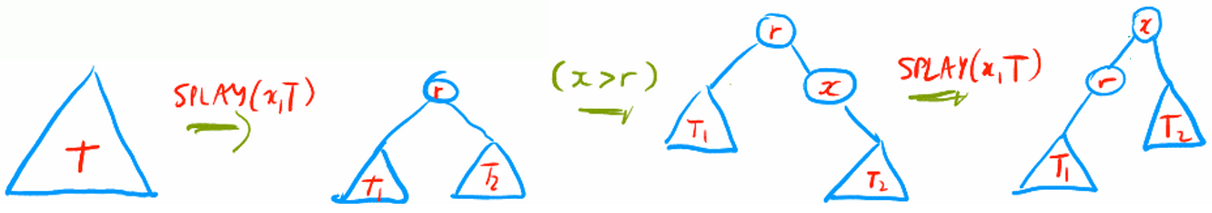
\includegraphics[width=0.8\linewidth]{Images/capitolo_1_2/splay_tree.png}
        \label{fig:splay_tree}
    \end{figure}
    \item \textbf{Delete(x,T)} Si effettua una Splay(x,T) e si cancella il nodo\footnote{Si ricordi che il nodo sarà la root dopo splay.} ottenendo quindi due alberi $T_1, T_2$. Si effettua nuovamente un splay(x, T) e, sia r la nuova radice, si ponga la radice di $T_2$ come figlio destro del nodo r.
\end{itemize}
\section{Analisi ammortizzata di Splay}
Consideriamo i cosi delle operazioni elementari che per zig è 1 mentre per zig-zag e zig-zig è 2. Poniamo
\begin{itemize}
    \item $S(\nu)=$\# nodi nel sotto albero con radice $\nu$;
    \item $R(\nu)= log(S(\nu))$ che chiameremo \textbf{rango di $\nu$};
    \item $\phi(T) = \sum_{\nu\in T} R(\nu)$;
\end{itemize}
\begin{figure}[H]
    \centering
    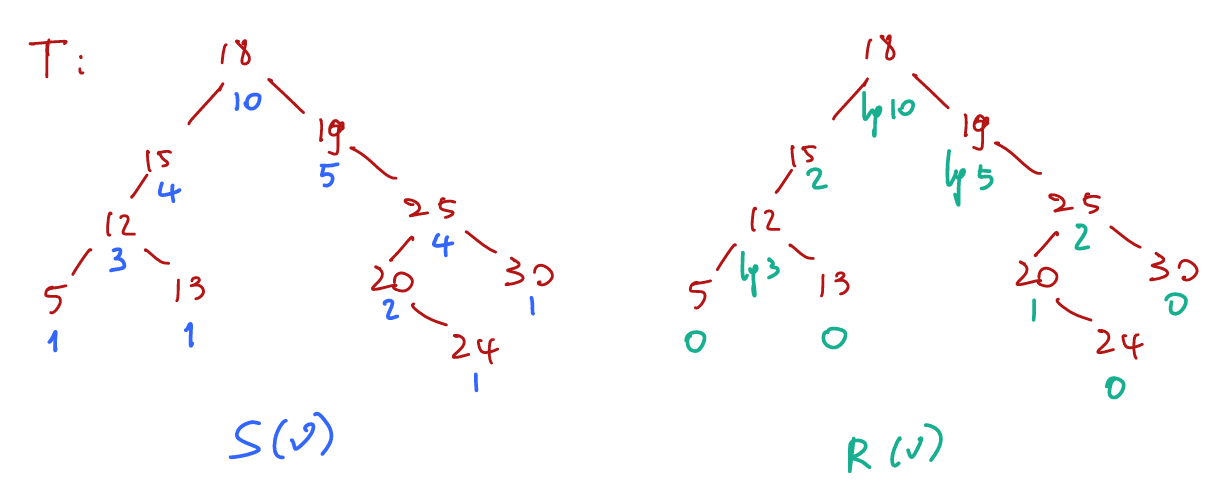
\includegraphics[width=0.8\linewidth]{Images/capitolo_1_2/rango_s_splay.png}
    \label{fig:rango_s}
\end{figure}

Sia $T_0$ un albero vuoto, avremo che $\phi(T_0) = 0$ e, sia T un albero qualsiasi, avremo che:
\[\phi(T)=\sum R(\nu)=\sum log(S(\nu)) \ge \phi(T_0)=0\]

Dunque sappiamo che possiamo utilizzare il metodo del potenziale per avere un upper bound al costo di M operazioni di cui N sono inserimenti su un albero inizialmente vuoto. 

\textbf{LEMMA}
Siano $a,b>0\quad c\ge a+b$ allora $log(a)+log(b)\leq2log(c)-2$. Possiamo dimostrarlo:
\begin{figure}[H]
    \centering
    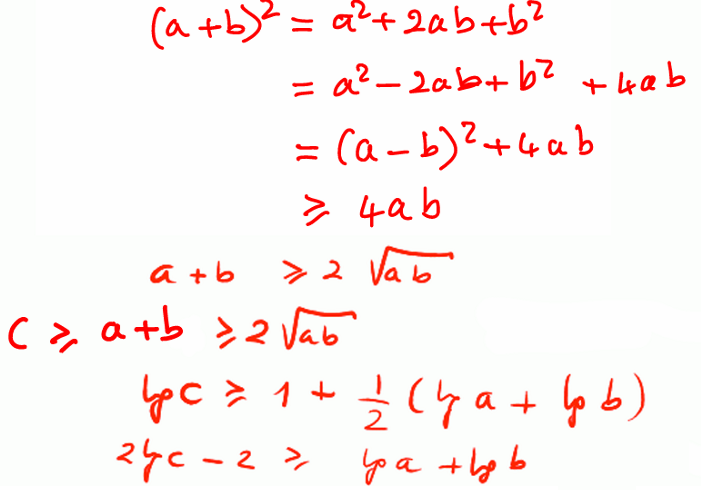
\includegraphics[width=0.5\linewidth]{Images/capitolo_1_2/dimostrazione_lemma.png}
    \label{fig:lemma_c_magg_a+b}
\end{figure}


Vediamo di dimostrare che il costo ammortizzato dell'operazione Splay(x, T) è al più $3(R(root(T))-R(x))+1$. Calcoliamo il costo ammortizzato di ogni operazione zig, zig-zag, zig-zig. Indicheremo con $S_i(x),S_f(x)$ il numero di nodi nel sotto-albero di radice x prima e dopo l'operazione. Allo stesso modo considereremo $R_i(x), R_f(x)$.

\textbf{Caso Zig}\\
Il costo reale di questa operazione è 1 poiché avviene solo una rotazione. Sappiamo che $\Delta\phi = R_f(x,p)-R_i(x,p)$ e osserviamo che:
\begin{figure}[H]
    \centering
    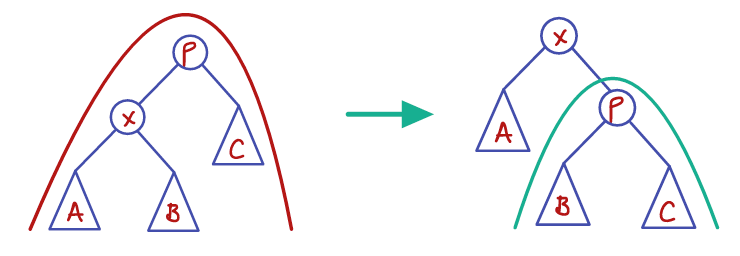
\includegraphics[width=0.5\linewidth]{Images/dimostrazione_zig_zigzag_zigzig/zig_1.png}
    \label{fig:zig_1}
\end{figure}
$S_f(p) \leq S_i(p) \xrightarrow{} R_f(p)\leq R_i(p) \xrightarrow{}\Delta\phi\leq R_f(p) - R_i(x) $\footnote{Visto che $\Delta\phi= (R_f(x)-R_f(p))+(R_f(p)-R_i(p))$ e che abbiamo visto che il rango iniziale è maggiore di quello finale, possiamo concludere che $R_f(p)-R_i(p)=0$.}\\
Osserviamo anche che, allo stesso modo, $S_i(x)\leq S_f(x) \xrightarrow{}R_i(x)\leq R_f(x) \xrightarrow{} R_f(x)-R_i(x) \geq0 \xrightarrow{}\Delta\phi\leq3(R_f(x)-R_i(x))$. Per cui, $c_{zig}' = 1+\Delta\phi \leq 1+3(R_f(x)-R_i(x))$\\
\begin{minipage}{\linewidth}
    \textbf{Caso Zig-Zig}\\
    Come abbiamo già detto, questa operazione ha costo reale 2. Qui i nodi coinvolti sono 3 per cui $\Delta\phi = R_f(x,p,g)-R_i(x,p,g)$. Analizziamo:
    \begin{figure}[H]
        \centering
        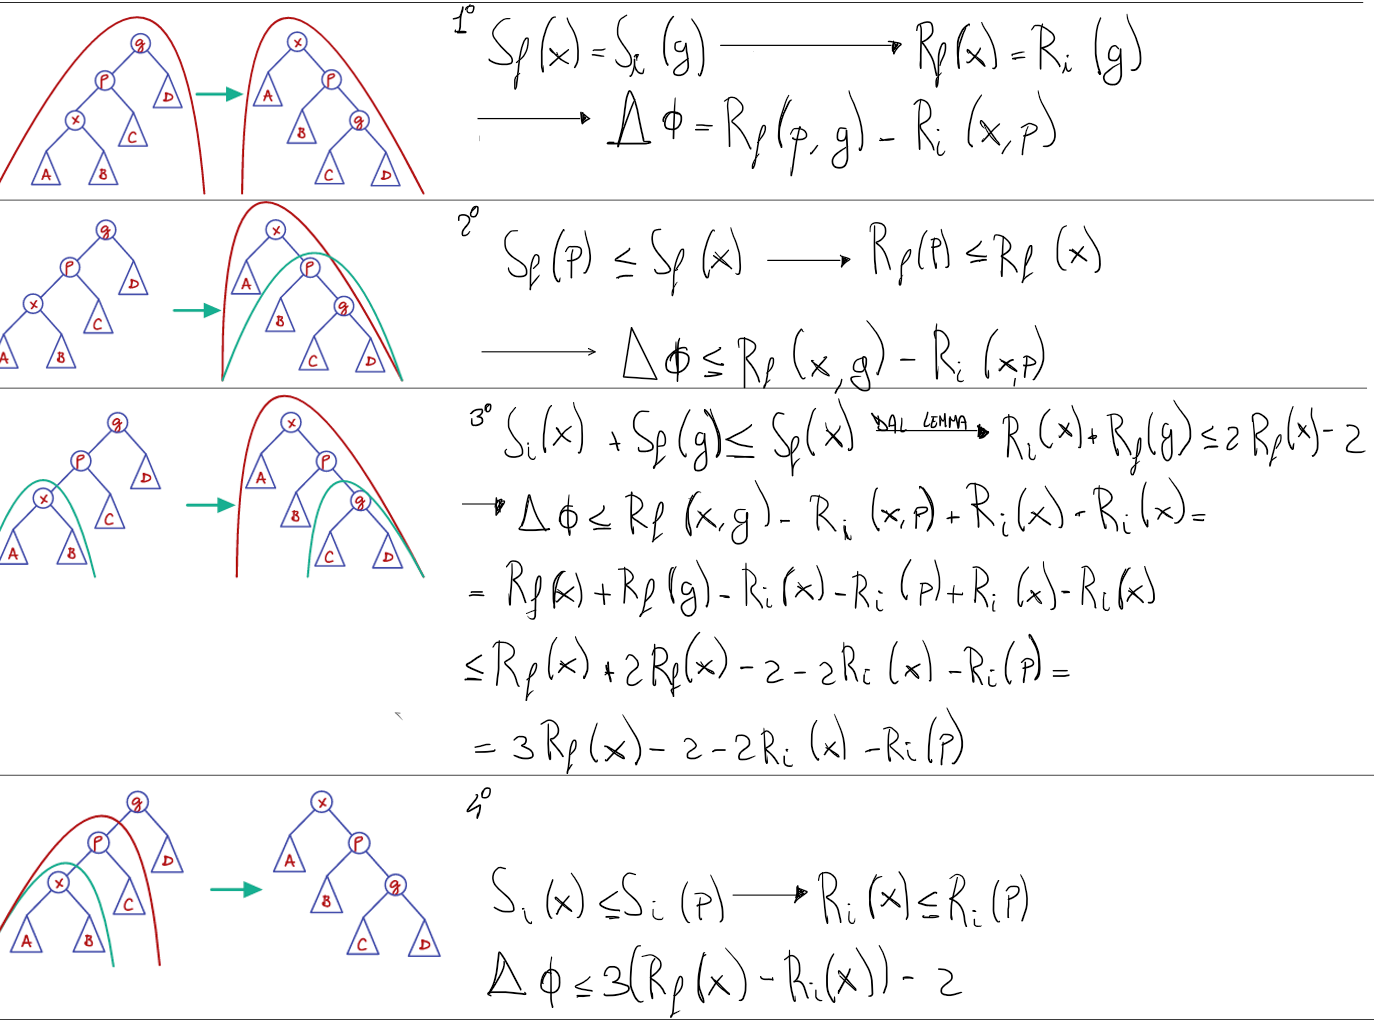
\includegraphics[width=1\linewidth]{Images/dimostrazione_zig_zigzag_zigzig/zig-zig_dimostrazione.png}
    \end{figure}
\end{minipage}
Per cui, alla fine di questa analisi possiamo concludere che $c_{zig-zig}'=2+\Delta\phi\leq3(R_f(x)-R_i(x))$\\

\textbf{Caso Zig-Zag}\\
Anche in questo caso, l'operazione reale ha costo 2 e sono coinvolti 3 nodi per cui $\Delta\phi = R_f(x,p,g)-R_i(x,p,g)$. 
Analizziamo:
\begin{figure}[H]
    \centering
    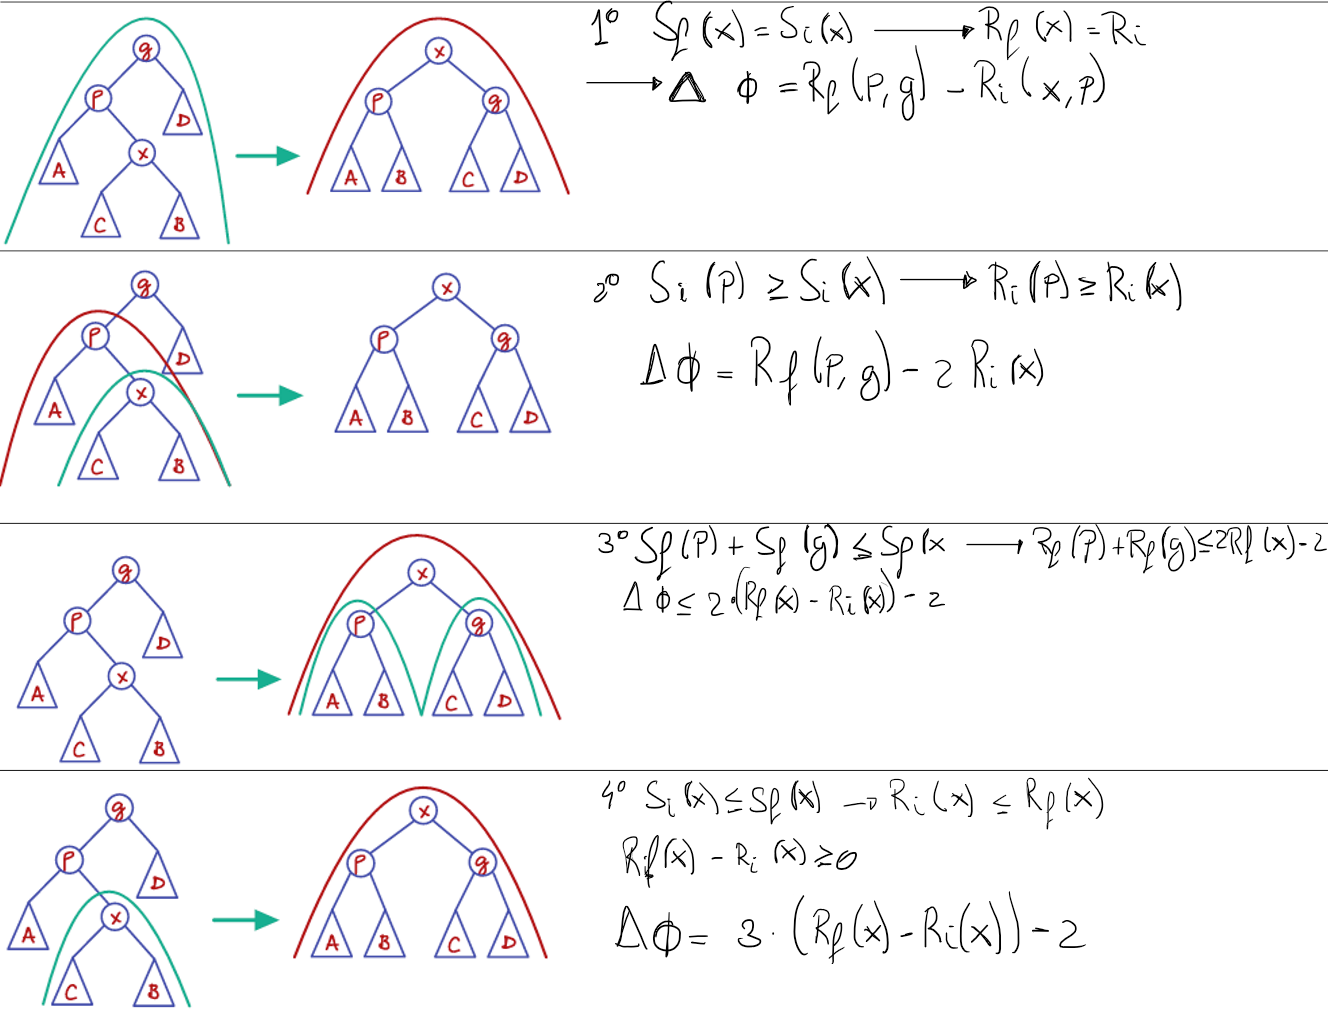
\includegraphics[width=1\linewidth]{Images/dimostrazione_zig_zigzag_zigzig/zig-zag.png}
\end{figure}
Da cui segue che, alla fine di questa analisi possiamo concludere che.

\[c_{zig-zag}'=2+\Delta\phi\leq3(R_f(x)-R_i(x))\]\\

Pertanto, posto splay(x) = $Z_1, Z_2,...,Zk$ con $Z_j \in{\text{zig, zig-zag,zig-zig}}$ avremo che:
\begin{itemize}
    \item $c_j'=$ costo ammortizzato dell'operazione $Z_j$;
    \item $R_i^j(x)=$ rango di x poco prima di $Z_j$;
    \item $R_f^j(x)=$ rando di x poco dopo $Z_j$.
\end{itemize}
Cerchiamo di calcolare $c_{splay}'$:
\begin{align*}
    &c'_{splay}=\sum_j^kc_j'\le \sum_j^k3(R_f^j(x)-R_i^j(x))+1\\
    &=\sum_j^k3(R_f^j(x)-R_f^{j-1}(x))+1\\
    &=3(R_f^k(x)-R_i^0(x))+1 = 3(R_f^k(x)-R_i^1(x)+1\\
    &=3(R_i^1(root(T))-R_i^1(x))+1 \quad \text{Root(T) = $R_f^k$ poiché x va poi sulla root}\\
    &=3(R(root(T))-R(x))+1 \quad \text{E, quindi...}\\\\
    &c_{splay}'\leq3(R(root(T))-R(x))+1
\end{align*}

Una sequenza di M operazioni di search, insert e delete sono $M'=O(M)$ operazioni di splay, ciascuna di costo ammortizzato $c_{splay}'\le3(R(root(T_j))-R(x_j))+1 \leq 3R(root(T_j))+1$. Posto che $N'$ sia il massimo numero di nodi nell'albero, avremo che $c_{splay}' \leq3R(root(Tj))+1\leq3log(N')+1$. Pertanto:
\[\sum_j^Mc_j=\sum_j^{M'}c_{splay_j}\leq\sum_j^{M'}c_{splay_j}'\leq M'(3log(N')+1)=O(Mlog(N')\]

Partendo da un albero inizialmente vuoto ed eseguendo N operazioni di inserimento tra le M si ha che una sequenza di M operazioni ha costo O(MlogN) cioè ogni operazione ha tempo ammortizzato logaritmico.

\section{Top-Down Splay Trees}
Il tipo di Splay Trees che abbiamo illustrato prima, si chiamano \textbf{bottom up splay trees}. Questi sono molto facili da implementare, tuttavia hanno alcuni problemi implementativi dato che le rotazioni danno luogo ad un bottom up e quindi occorre memorizzare il cammino dalla radice al nodo oppure mantenere per ciascun elemento il nodo padre.

La variante che risolve questo problema si chiama Top-Down e, mantenendo il costo logaritmico, risolve questo problema. L'idea è che mentre si procede alla ricerca, si trattano tutti i nodi incontrati. Ogni opearzione di splay dividerà l'albero in tre parti:
\begin{enumerate}
    \item L(eft): l'albero di sinistra che ha tutti i nodi più piccoli rispetto ad x;
    \item $T'$: l'albero centrale su cui si continua la ricerca;
    \item R(ight): l'albero di destra per cui tutti i nodi sono più grandi rispetto ad x; 
\end{enumerate}

Inizialmente x è la radice dell'albero T e L e R sono vuoti. Una volta scesi di due o uno, applichiamo l'operazione di zig-zag, zig-zig o zig e aggiorniamo i tre alberi L, T' e R mantenendo la proprietà $L\leq T'\leq R$. Alla fine gli alberi saranno riordinati come segue:
\begin{figure}[H]
    \centering
    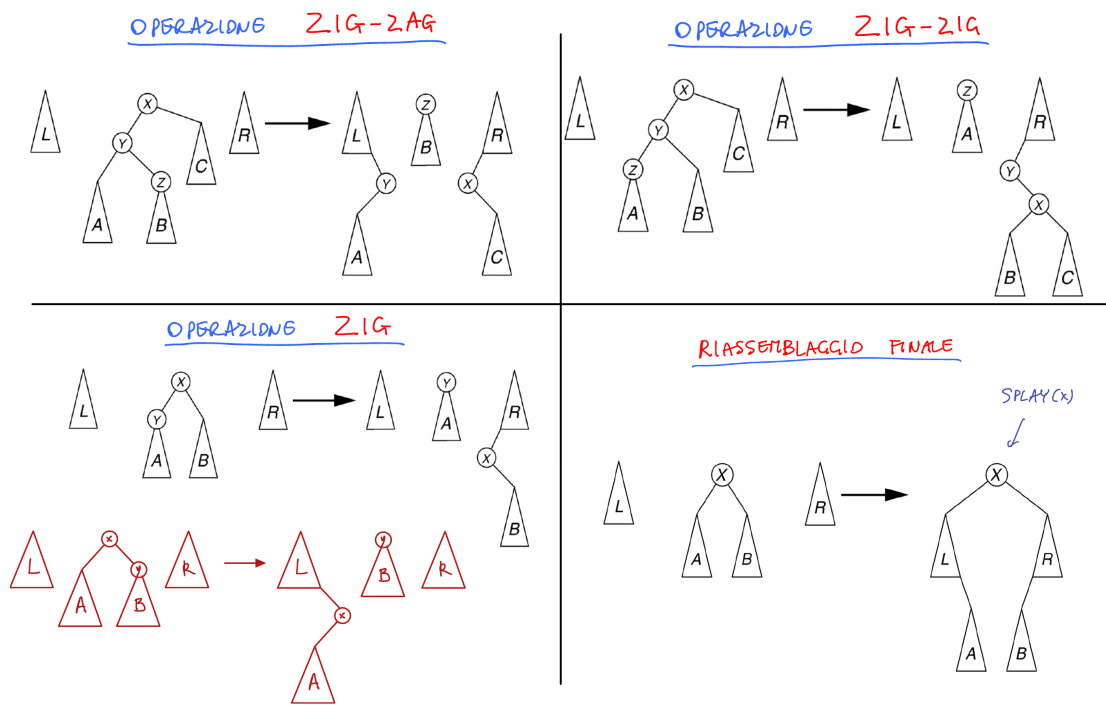
\includegraphics[width=1\linewidth]{Images/top-down_tree/totale.png}
    \label{fig:schema_top_down}
\end{figure}